\pgfplotsset{compat=1.3,
    %legend drawing style, single bar instead of the default double mini bars
    /pgfplots/ybar legend/.append style={ 
        /pgfplots/legend image code/.code={%
           \draw[##1,/tikz/.cd,yshift=-0.25em]
           (0cm,0cm) rectangle (7pt,0.8em);
        },
    }
}

%%sharp linear plots
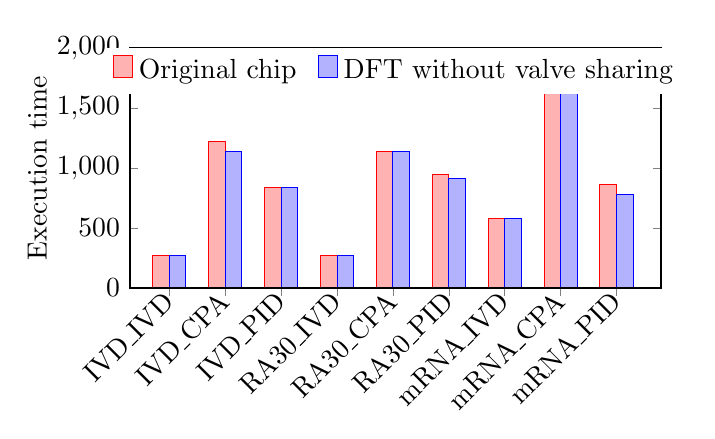
\begin{tikzpicture}
%remove space surrounding text nodes and the whole picture caused by text
%[every node/.style={inner sep=0,outer sep=0}]

%\pgfplotstableread{
%$chip  timebefore  timeafter
%1        9         25          
%2        62        103            
%3        51        168            
%4        43         90            
%5        74        137            
%6        95        171          
%7        102       140            
%8        107       160
%9        174       214
%10       138       256
            
%}\loadedtable

\pgfplotstableread{
chip timebefore timeafter
1 270	270
2 1220	1140
3 840	840
4 270	270
5 1140	1140
6 950	910
7 580	580
8 1640	1640
9 860	780




}\loadedtable

\begin{axis}[
%xaxis styles
%xticklabels={s5378,s9234, s13207, s15850, s38584,systemcdes, mem\_ctrl, usb\_funct, ac97\_ctr, pci\_bridge32}, 
xticklabels={IVD\_IVD, IVD\_CPA, IVD\_PID, RA30\_IVD,RA30\_CPA, RA30\_PID, mRNA\_IVD, mRNA\_CPA, mRNA\_PID}, 
xtick={1,...,9},
%x axis limits
xmin=0.3, xmax=9.8,
%x and y axes scaling
%x=0.763cm, y=0.18cm,
x=0.71cm, y=0.0152mm, 
x tick label style={rotate=45, xshift=0pt,yshift=0pt,anchor=east, 
%"iner sep" removes the space surrounding label tick texts at the bottom,
%so that there is no useless white space at the lower boundary of the picture. The
%space of tick label texts need to be removed because they are the lowest
%units without an xlable
inner sep=0}, 
xticklabel pos=left, xtick align=outside, xtick pos=left,
%
%y axis limits
ymin=0, ymax=2000,
%yaxis styles
ylabel={Execution time}, 
%"inner sep" for ylabel removes the white space on the leftmost edge of the picture
ylabel style={inner sep=0}, 
ylabel shift=0pt, ytickmin=0,ytickmax=2000, 
%
%legend styles
legend columns=3, 
legend style={
at={(0.5,0.907)}, anchor=center, 
%column separation between legend items
/tikz/every even column/.append style={column sep=0.2cm},
%distance between legend symbols and text nodes
%column sep=2.5cm,
%space surrounding the text boxes in legend
%nodes={inner xsep=20pt},
%no stroke in legend
draw=none, 
},
%
%axis drawing line width
line width=0.75pt,
%space between the bars in a group
ybar=0pt, 
bar width=6pt,
%axis on top makes the bars drawn on a layer below axis lines. Otherwise, the bottom lines of the
%bars can be seen with different colors on the bottom axis line.
axis on top=true,
major tick length=3pt,
]  
\addplot[ybar, line width=0.35pt, red, fill=red!30!white] table[x=chip,y=timebefore] {\loadedtable};
%\addplot[ybar, line width=0.35pt, brown!60!black, fill=brown!30!white] table[x=chip,y=Multiplex] {\loadedtable};
\addplot[ybar, line width=0.35pt, blue, fill=blue!30!white] table[x=chip,y=timeafter] {\loadedtable};
\legend{Original chip, DFT without valve sharing}

\end{axis}
\end{tikzpicture}
